\section{Building Models}
\label{sec:component_diagrams-buildingModels}

A CODA model is an Event-B model with component models as child elements of Event-B machines. Therefore, the first step is to create an Event-B project with an Event-B machine in it. To add a component model, right click on the Event-B machine and from the context menu (Figure \ref{fig:AddingaComponentModeltoaMachine}), select \textbf{\texttt{Add Component}}, and provide a name for the top-level component. Note that component models exist within components; therefore the top-level element is a single \emph{root} component which will contain the component model.
 

\begin{figure}[!htbp]
  \centering
  \ifplastex
  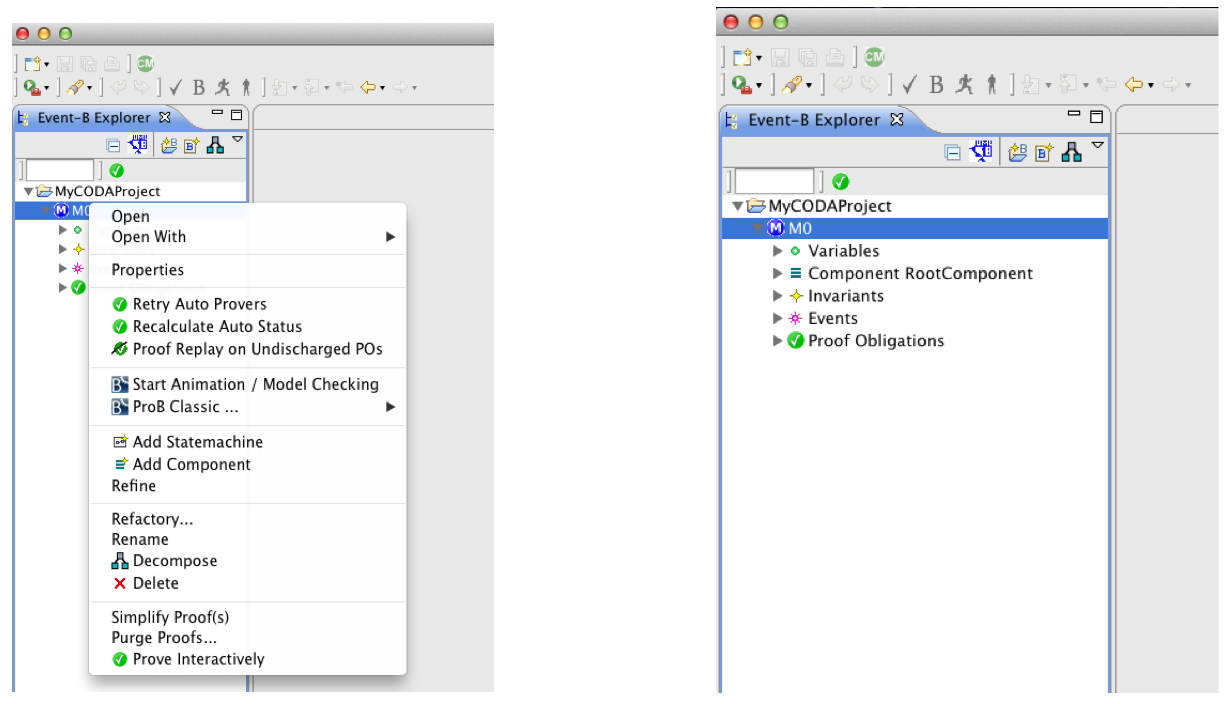
\includegraphics[width=768]{figures/image4.png}
  \else
  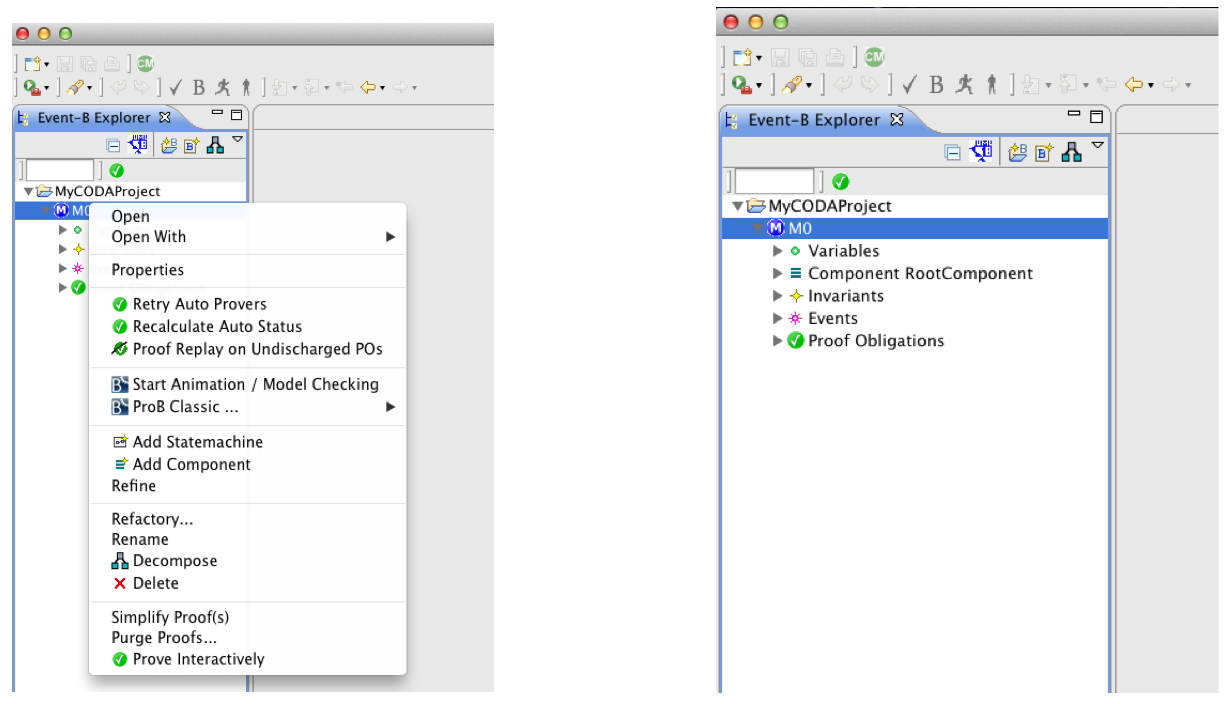
\includegraphics[width=0.75\textwidth]{figures/image4.png}
  \fi
  \caption{Adding a Component Model to a Machine}
  \label{fig:AddingaComponentModeltoaMachine}
\end{figure}


The component can now be opened for editing with the Component Diagram editor (Figure \ref{fig:TheComponentDiagramEditor}) by double clicking on it in the navigator tree.
 
\begin{figure}[!htbp]
  \centering
  \ifplastex
  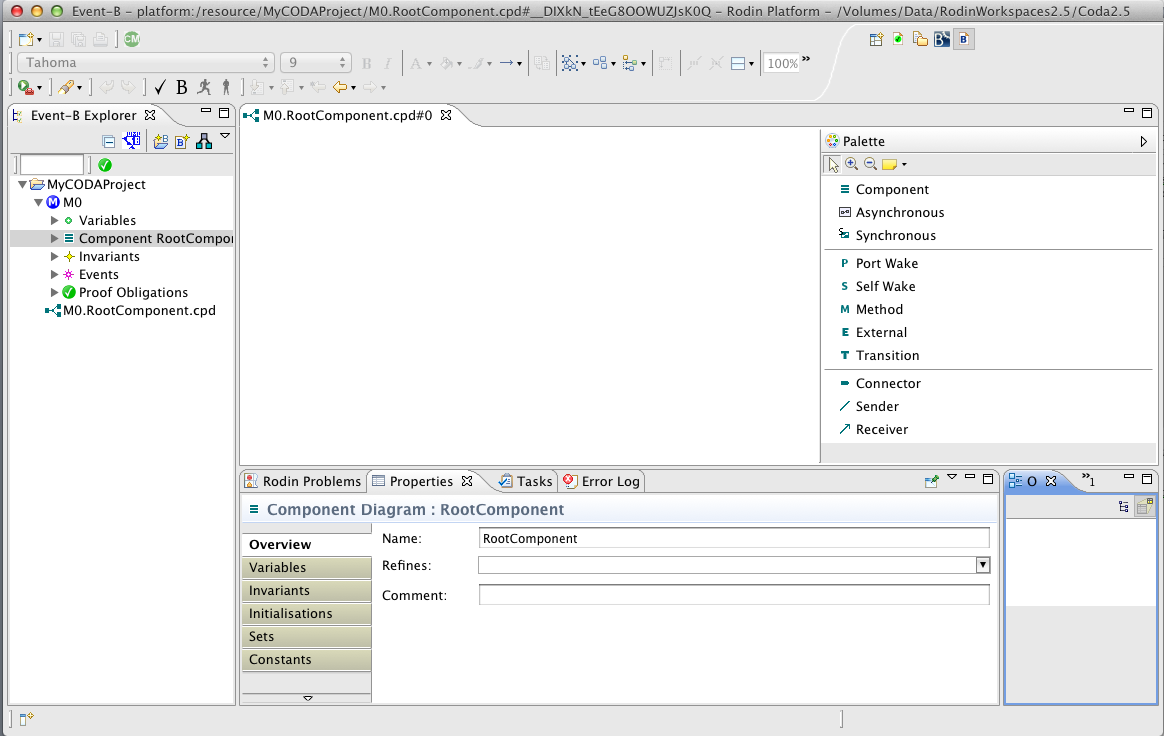
\includegraphics[width=1024]{figures/image5.png}
  \else
  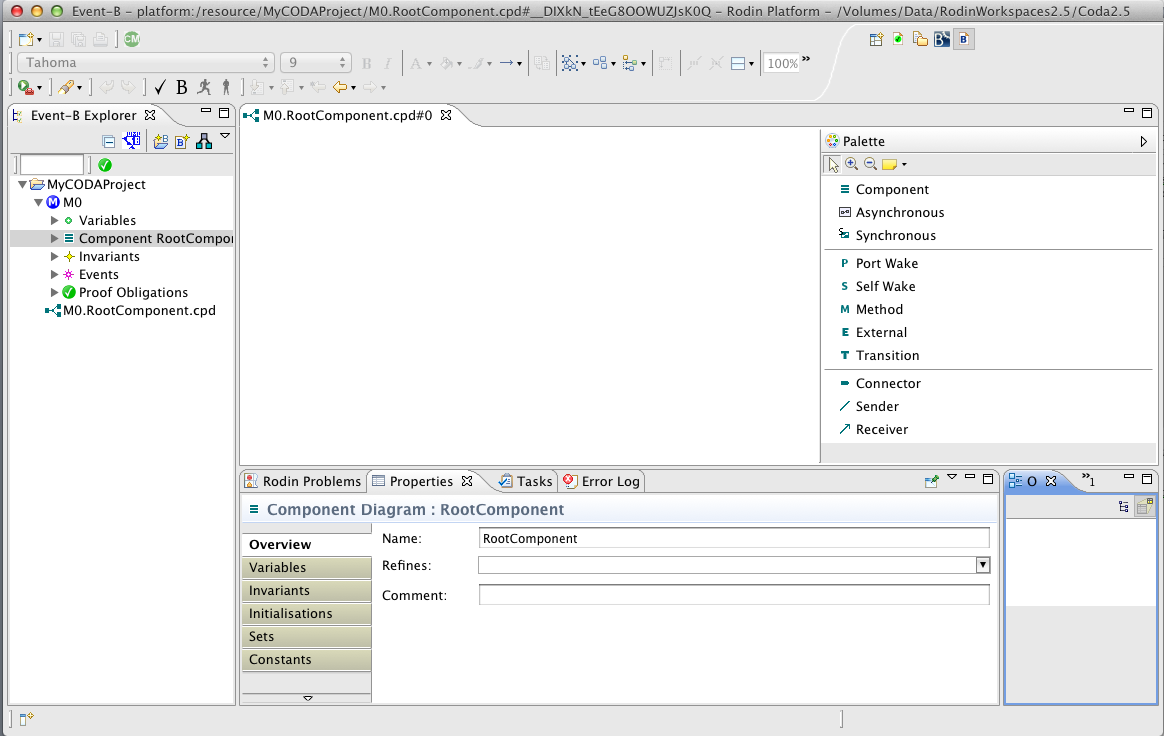
\includegraphics[width=1.0\textwidth]{figures/image5.png}
  \fi
  \caption{The Component Diagram Editor !!!TBD!!! THIS DIAGRAM SHOULD HAVE ANNOTATIONS - SEE WORD VERSION}
  \label{fig:TheComponentDiagramEditor}
\end{figure}


A component is created by clicking the Component item in the tool palette and then clicking on the canvas in the desired position for the component. (N.b. do not hold the mouse button on while doing this, just click and let go). Name the component either on the diagram or in the properties sheet name field.


A connector channel is created in a similar way. A link should be added to indicate which component sends on the connector. This is done by clicking on the Sender item in the tool palette and then click \& hold on the connector and dragging the link to the sending component. Similarly links can be added to indicate the receivers of the connector. (In both cases the link must be started from the connector and finished at a component).


Operations are added to a component by clicking on one of the tool palette operations and then clicking in the operations container of the parent component (Figure \ref{fig:Adding an Operation to a Component}). The different kinds of operation are briefly introduced in this section and illustrated in more detail in the tutorial section. Note that operations cannot be named because they derive their labels from the name of the events that they elaborate. The event elaboration property must be set in the properties editor using either the Add Event button (to link to an existing event) or the Create \& Add button to create a new event and link to it).


CODA models are based on Event-B and must be converted into equivalent Event-B models in order to perform verification. The Event-B generator is run by clicking the \textbf{B} icon in the toolbar menu (see Figure \ref{fig:TheComponentDiagramEditor}).


Event-B models consist of events that perform actions when their guards are true. CODA operations contribute guards and actions to an event that already exists in the underlying Event-B model. Operations may have ordinary guards and actions expressed in the Event-B notation but they may also have special kinds of guards and actions that are appropriate for the component modelling language. Furthermore, the operations themselves are specialised into several kinds for the component modelling language, which requires further guards and actions to be generated in the underlying Event-B. The following paragraphs introduce the specialised kinds of operations and the specialised kinds of guards and actions.
 
 \begin{figure}[!htbp]
  \centering
  \ifplastex
  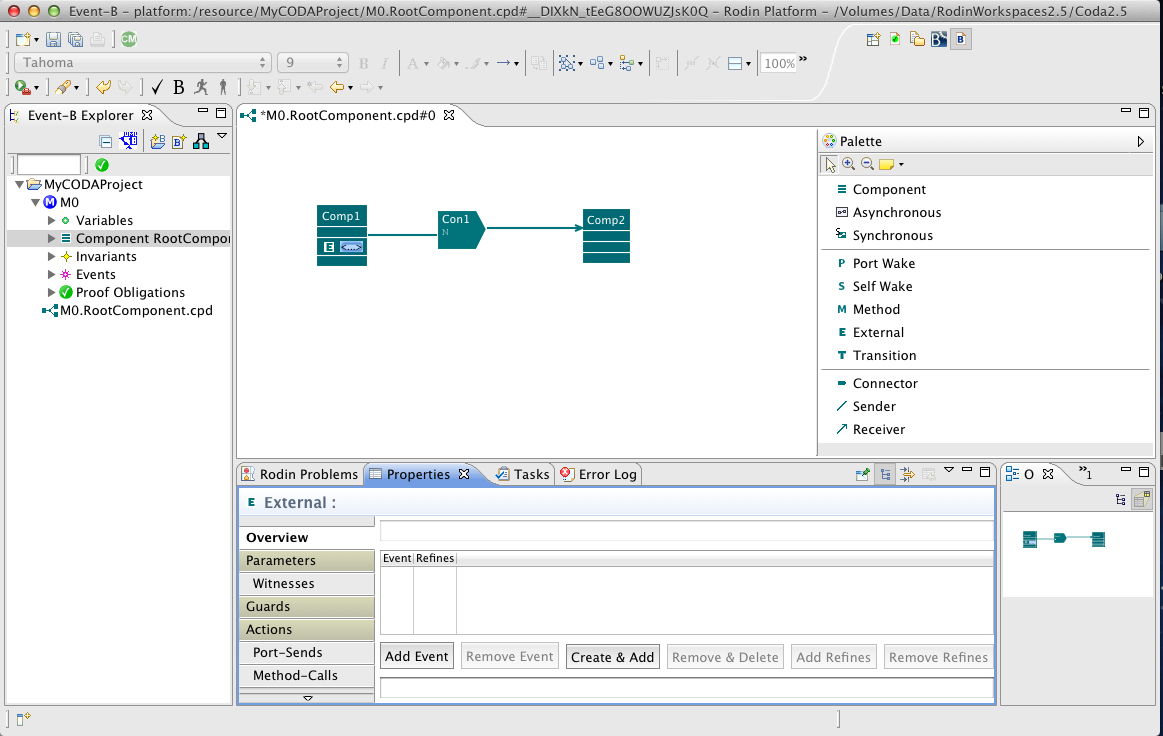
\includegraphics[width=768]{figures/image6.png}
  \else
  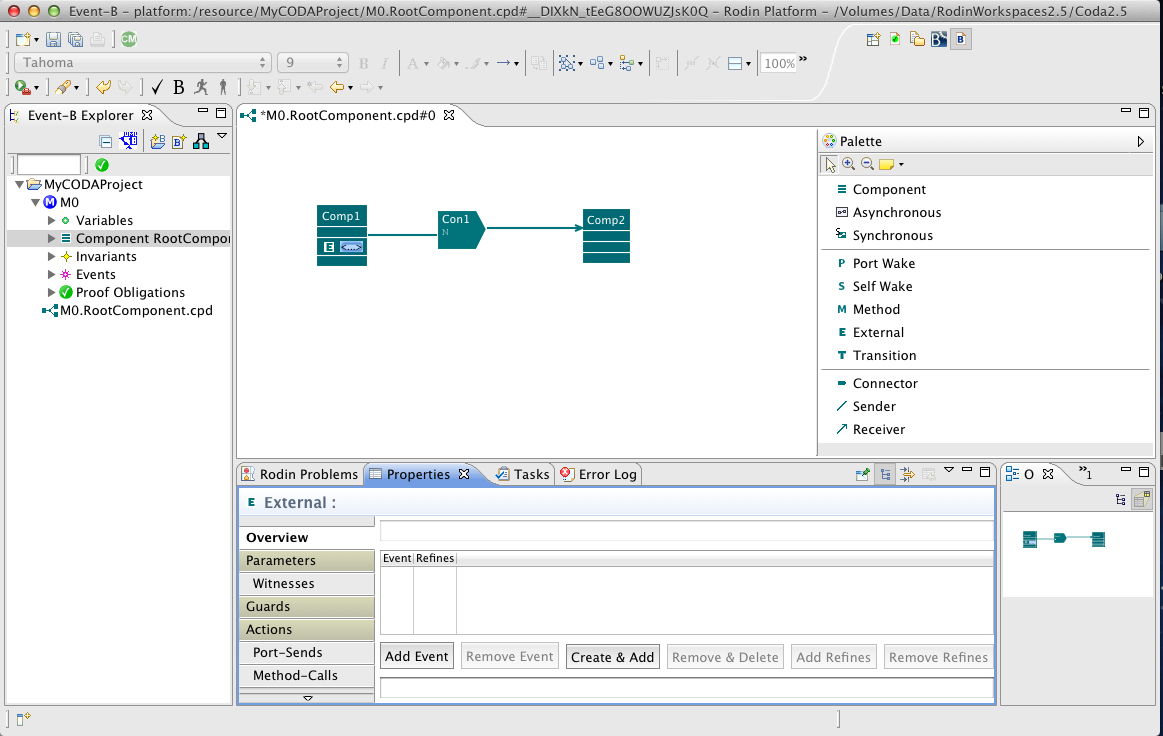
\includegraphics[width=0.75\textwidth]{figures/image6.png}
  \fi
  \caption{Adding an Operation to a Component}
  \label{fig:Adding an Operation to a Component}
\end{figure}


Having created operations they can be configured to send and receive on the connectors by adding port-send actions (Figure \ref{fig:AddingaSendActiontoanOperation}) and port-wake operations with port-wake guards. A port-send action represents the action of sending data over a connector and can be added to any operation in a component that has an outgoing connection to the connector. A port-wake operation is needed in the receiving component of the connector in order to respond to the receipt of data on the connector. These port-wake operations must have port-wake guards that define what connector data they respond to. 


\begin{figure}[!htbp]
  \centering
  \ifplastex
  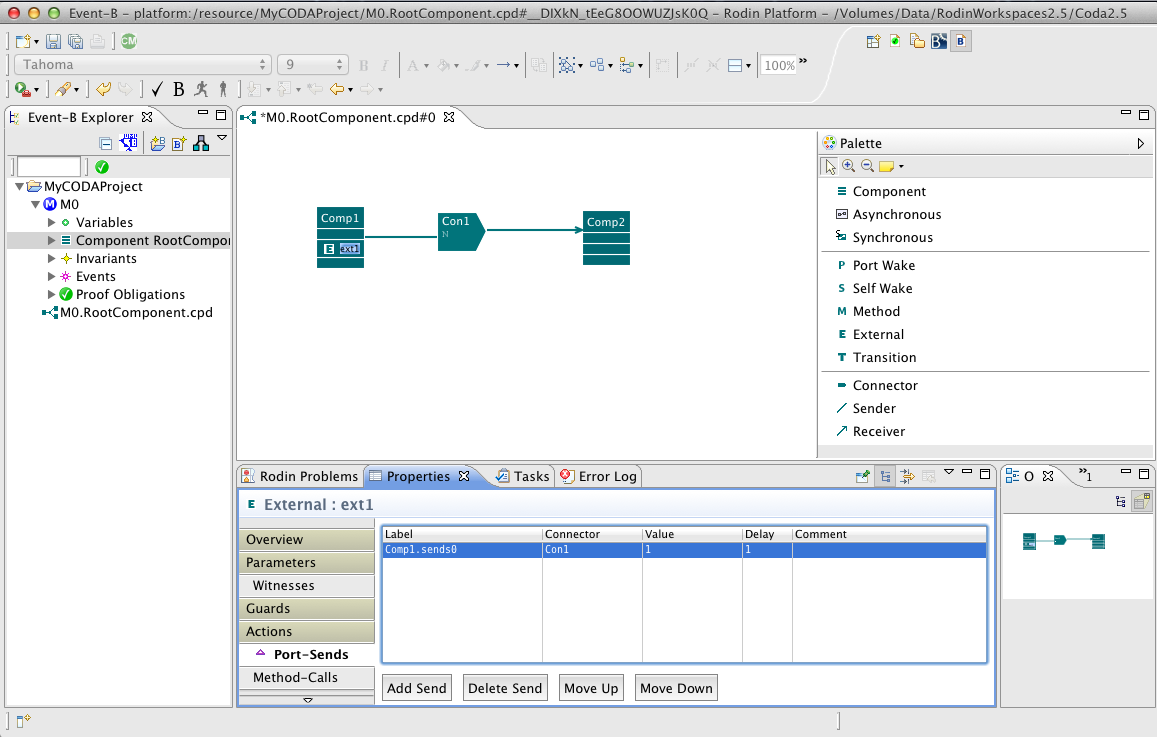
\includegraphics[width=768]{figures/image7.png}
  \else
  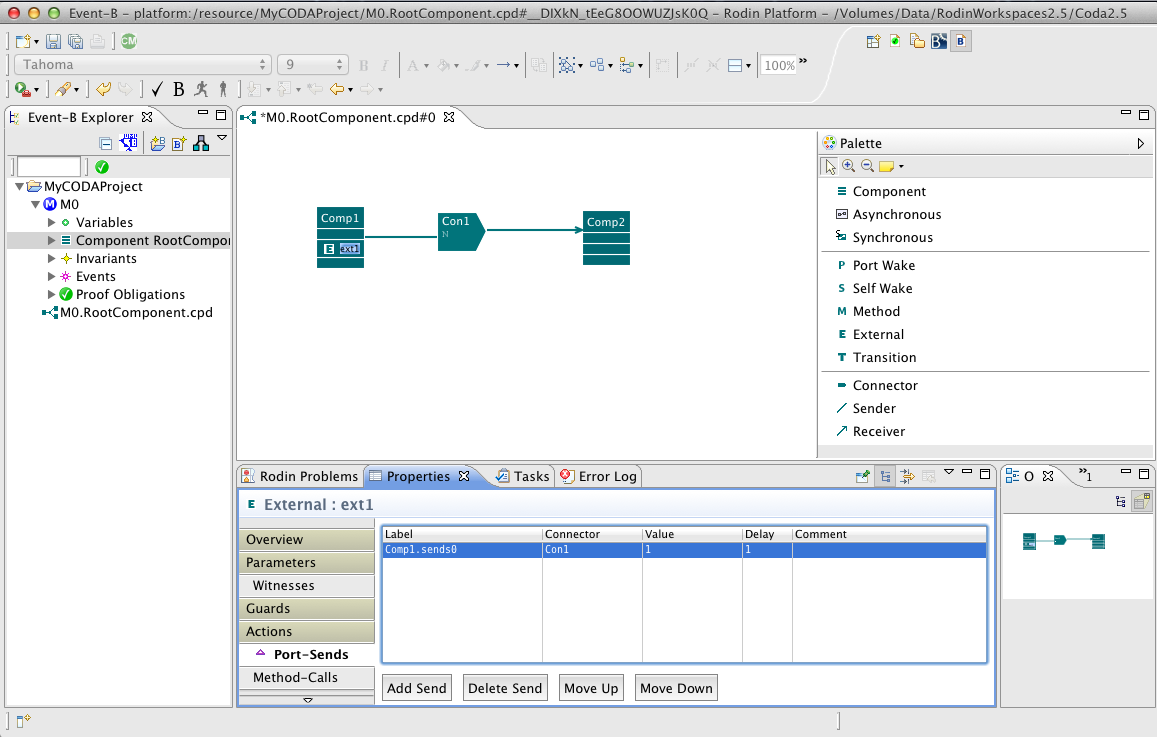
\includegraphics[width=0.75\textwidth]{figures/image7.png}
  \fi
  \caption{Adding a Send Action to an Operation}
  \label{fig:AddingaSendActiontoanOperation}
\end{figure}
 
 
Similarly, self-wake actions can be added to any operation and self-wake operations must be added to service them. A self-wake action represents the scheduling of a component wake-up at some future time and can be added to any operation in a component. A self-wake operation is needed in the component to respond to the component wake-up. 


Method call actions can be added to operations and method operations must be added to service the calls. A method call action immediately enables a particular method operation, which must then complete within the same clock cycle.


External operations represent events that occur in the environment that the model must respond to. The timing of these events is uncontrolled and therefore not synchronised to the clock in any way. These events may perform any of the operation actions (port-wake, self-wake, method calls) described here.


Data can be defined in the properties by selecting a component that represents the scope of the data (currently this scoping is not enforced). Note that the diagram canvas represents a root component and this may be the most appropriate place for global data. If any sets, constants or axioms are defined in this way an Event-B Context will be automatically generated to contain them.



State-machines may be added to components. Double clicking on the state-machine icon/name in the component opens a state-machine diagram. Since the state-machine diagram is a standard Rodin plugin (rather than part of the CODA specific tool) component behaviour such as port sends etc. cannot be added on the state-machine transitions. For this reason a special kind of component operation (Transition) is available in the component diagram. Transition operations must link to an event that is also linked to a state-machine transition. They enable component behaviour to be added to the components state-machine transitions. 


Two kinds of state-machine are available. Asynchronous state-machines are not linked to the clock whereas synchronous state-machines are tightly linked to the clock so that, while enabled, only one transition may be taken on each clock tick.




%%% Local Variables:
%%% mode: latex
%%% TeX-master: "component_diagrams-user_manual"
%%% End:
